\documentclass[ignorenonframetext,]{beamer}
\setbeamertemplate{caption}[numbered]
\setbeamertemplate{caption label separator}{: }
\setbeamercolor{caption name}{fg=normal text.fg}
\beamertemplatenavigationsymbolsempty
\usepackage{lmodern}
\usepackage{amssymb,amsmath}
\usepackage{ifxetex,ifluatex}
\usepackage{fixltx2e} % provides \textsubscript
\ifnum 0\ifxetex 1\fi\ifluatex 1\fi=0 % if pdftex
  \usepackage[T1]{fontenc}
  \usepackage[utf8]{inputenc}
\else % if luatex or xelatex
  \ifxetex
    \usepackage{mathspec}
  \else
    \usepackage{fontspec}
  \fi
  \defaultfontfeatures{Ligatures=TeX,Scale=MatchLowercase}
\fi
\usetheme[]{Boadilla}
% use upquote if available, for straight quotes in verbatim environments
\IfFileExists{upquote.sty}{\usepackage{upquote}}{}
% use microtype if available
\IfFileExists{microtype.sty}{%
\usepackage{microtype}
\UseMicrotypeSet[protrusion]{basicmath} % disable protrusion for tt fonts
}{}
\newif\ifbibliography
\hypersetup{
            pdftitle={Rules of Probability},
            pdfauthor={Chris Che-Castaldo, Mary B. Collins, N. Thompson Hobbs},
            pdfborder={0 0 0},
            breaklinks=true}
\urlstyle{same}  % don't use monospace font for urls

% Prevent slide breaks in the middle of a paragraph:
\widowpenalties 1 10000
\raggedbottom

\AtBeginPart{
  \let\insertpartnumber\relax
  \let\partname\relax
  \frame{\partpage}
}
\AtBeginSection{
  \ifbibliography
  \else
    \let\insertsectionnumber\relax
    \let\sectionname\relax
    \frame{\sectionpage}
  \fi
}
\AtBeginSubsection{
  \let\insertsubsectionnumber\relax
  \let\subsectionname\relax
  \frame{\subsectionpage}
}

\setlength{\parindent}{0pt}
\setlength{\parskip}{6pt plus 2pt minus 1pt}
\setlength{\emergencystretch}{3em}  % prevent overfull lines
\providecommand{\tightlist}{%
  \setlength{\itemsep}{0pt}\setlength{\parskip}{0pt}}
\setcounter{secnumdepth}{0}
\usepackage{bm}
\usepackage{amsmath}
\usepackage{amssymb}
\usepackage{mathptmx}
\usepackage{nicefrac}
\usepackage{hyperref}
\usepackage{mathtools}
\usepackage{pgfpages}
\usepackage[mathscr]{euscript}
 \usepackage{tikz}

\setbeamersize{text margin left=10pt, text margin right=20pt}

\AtBeginSection[]{}

\setbeamertemplate{headline}{%
\leavevmode%
  \hbox{%
    \begin{beamercolorbox}[wd=\paperwidth,ht=2.5ex,dp=1ex]{author in head/foot}%
    \insertsectionnavigationhorizontal{\paperwidth}{}{\hskip0pt plus1filll}
    \end{beamercolorbox}%
  }
}

\setbeamertemplate{footline}
{
  \leavevmode%
  \hbox{%
  \begin{beamercolorbox}[wd=.3\paperwidth,ht=2.25ex,dp=1ex,center]{author in head/foot}%
    \usebeamerfont{author in head/foot}Che-Castaldo, Collins, Hobbs
  \end{beamercolorbox}%
  \begin{beamercolorbox}[wd=.6\paperwidth,ht=2.25ex,dp=1ex,center]{title in head/foot}%
    \usebeamerfont{title in head/foot}\insertshorttitle, \insertdate
  \end{beamercolorbox}%
  \begin{beamercolorbox}[wd=.1\paperwidth,ht=2.25ex,dp=1ex,center]{date in head/foot}%
    \insertframenumber{} / \inserttotalframenumber\hspace*{1ex}
  \end{beamercolorbox}}%
  \vskip0pt%
}

\makeatletter
\setbeamertemplate{navigation symbols}{}

\titlegraphic{\includegraphics[width=3cm]{../../Headers/Logo.png}}

%\setbeameroption{show notes}
%\setbeameroption{show notes on second screen=right}

\title{Rules of Probability}
\subtitle{Bayesian Modeling for Socio-Environmental Data}
\author{Chris Che-Castaldo, Mary B. Collins, N. Thompson Hobbs}
\date{August 2017}

\begin{document}
\frame{\titlepage}

\begin{frame}{Road map}

\begin{itemize}
\tightlist
\item
  Rules of probability

  \begin{itemize}
  \tightlist
  \item
    Conditional probability
  \item
    Independence
  \item
    The law of total probability
  \end{itemize}
\item
  Factoring joint probabilities
\end{itemize}

\end{frame}

\section{Rules of probability}\label{rules-of-probability}

\begin{frame}{Why do we need to know this stuff?}

\begin{enumerate}
\def\labelenumi{\arabic{enumi}.}
\tightlist
\item
  \textbf{Conditional probability} foundational for all the inferences
  that we make.
\item
  \textbf{The law of total probability} is the denominator of Bayes'
  Theorem.
\item
  \textbf{Factoring} joint distributions is how we deal with complexity,
  reducing high dimensional problems.
\item
  \textbf{Independence} allows us to simplify fully factored joint
  distributions.
\item
  Bayesian inference is based on \textbf{marginal distributions} of
  unobserved quantities.
\end{enumerate}

\end{frame}

\begin{frame}{Random variables:}

\begin{itemize}
\tightlist
\item
  are quantities governed by chance.
\item
  have a specific value called an \emph{events} or \emph{outcomes}.
\item
  are summarized by probability distributions.
\end{itemize}

Bayesians treat every unobserved quantity as a random variable.

\end{frame}

\begin{frame}{S=Sample Space}

\begin{itemize}
\tightlist
\item
  The set of all possible events or outcomes of an experiment or survey.
\item
  The sample space, \(S\) has a specific area.
\end{itemize}

\center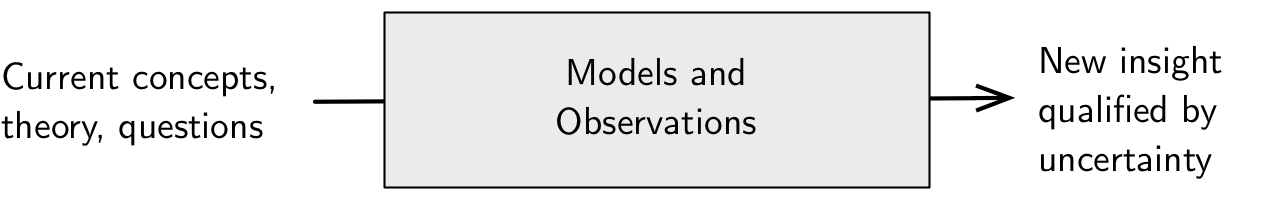
\includegraphics[width=0.95\paperwidth]{../../Graphics/ConceptsTheory.png}

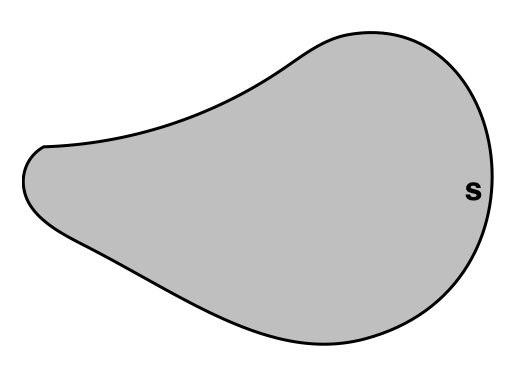
\includegraphics[height=1.25in]{S.png}

\end{frame}

\begin{frame}{Events in S}

\begin{itemize}
\tightlist
\item
  Can define and event, \(A\).
\item
  The area of event \(A\) is less than \(S\).
\end{itemize}

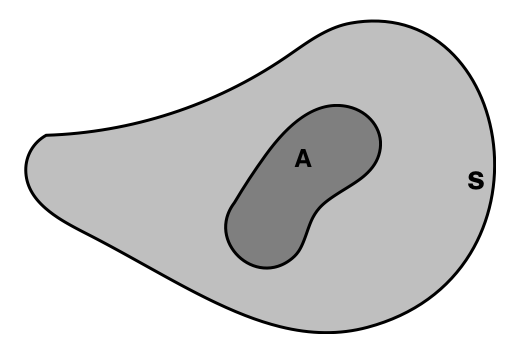
\includegraphics[height=1.25in]{eventA.png}

\end{frame}

\begin{frame}{What is the probability of event A?}

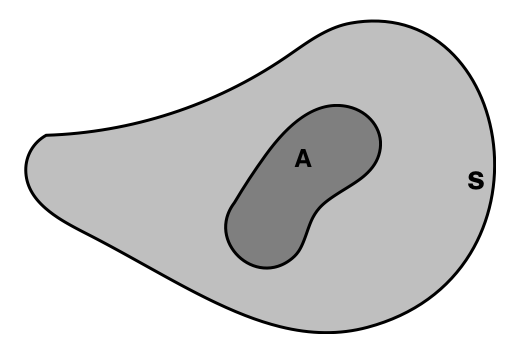
\includegraphics[height=1.25in]{eventA.png}

\(\Pr(A) = \frac{\text{Area of}~A}{\text{Area of}~S}\)

\end{frame}

\begin{frame}{Conditional Probability}

\emph{Conditional probability}: the probability of an event given that
\emph{we know} another event has occurred.

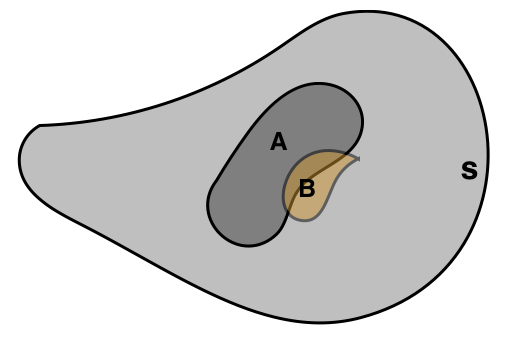
\includegraphics[height=1.25in]{eventB.png}

\end{frame}

\begin{frame}{What is the probability of event \(B\), given that event
\(A\) has occurred?}

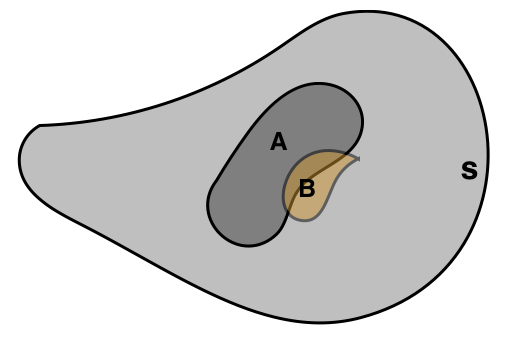
\includegraphics[height=1.25in]{eventB.png}

\(\Pr(B|A)\) = probability of \(B\) conditional on knowing \(A\) has
occurred

\end{frame}

\begin{frame}{What is the probability of event \(B\), given that event
\(A\) has occurred?}

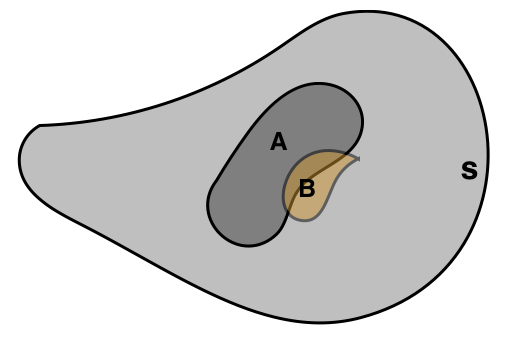
\includegraphics[height=1.25in]{eventB.png}

\(Pr(B|A) = \frac{\text{Joint Probability}}{\text{Probability of A}}=\frac{\Pr(A,B)} {\Pr(A)}\)

\end{frame}

\begin{frame}{What about the probability of event \(B\), given that two
other events have occured, events \(A\) and \(C\)?}

\(Pr(B|A,C) = \frac{\Pr(A,B,C)} {\Pr(A)}\)

\end{frame}

\begin{frame}{If the occurance of event A does not tell us anything
about event B?}

\emph{In this case, events A and B are said to be \textbf{independent}}

\end{frame}

\begin{frame}{Events are independent if and only if\ldots{}}

\(\Pr(A|B) = \Pr(A)\)

\end{frame}

\begin{frame}{Assuming independence, the joint probability of event A
and event B}

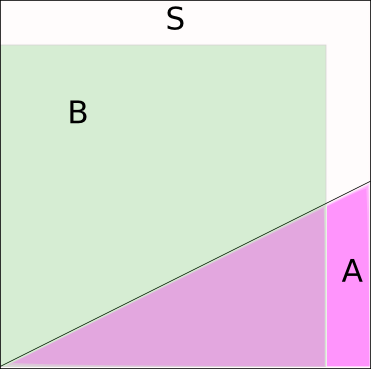
\includegraphics[height=2.25in]{rect3823.png}

\(\Pr(A,B) = \Pr(A) \Pr(B)\)

\end{frame}

\begin{frame}{The Law of Total Probability}

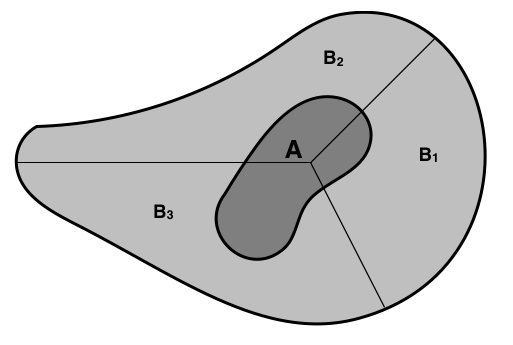
\includegraphics[height=1.25in]{totalProb.png}

We can define a set of events \(\{B_n : n = 1,2,3,...\}\), which taken
together define the entire sample space, \(\sum_n B_n = S\).

\end{frame}

\begin{frame}{What is the probability of event A?}

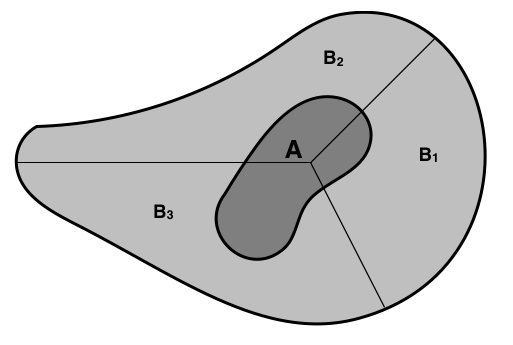
\includegraphics[height=1.25in]{totalProb.png}

\(\Pr(A) = \sum_n \Pr(A|B_n)\Pr(B_n)\) (discrete case)

\(\Pr(A) = \int \Pr(A|B)\Pr(B) dB\) (continuous case)

\end{frame}

\begin{frame}{The Chain Rule of Probability}

The chain rule of probability allows us to calculate any number of joint
distributions using only conditional probabilities. \vspace{1cm}

\(\Pr(z_1,z_2,...,z_n) = \Pr(z_n|z_{n-1},...,z_1) ... \Pr(z_3|z_2,z_1)\Pr(z_2|z_1)\Pr(z_1)\)

\vspace{1cm} Notice the pattern here.

\begin{itemize}
\tightlist
\item
  z's can be scalars or vectors.
\item
  Sequence of conditioning doesn't matter.
\item
  When we build models, we choose a sequence that makes sense.
\end{itemize}

\end{frame}

\begin{frame}{}

Chain rule of probability board work and independence

\end{frame}

\begin{frame}{Factoring joint probabilities}

Why is factoring useful?

\begin{itemize}
\tightlist
\item
  The rules of probability allow us to simplify complicated joint
  distributions, breaking them down into chunks.
\item
  Chunks can be analyzed one at a time.
\item
  Provide a usable graphical and mathematical foundation,
  \emph{critical} for the model specification step.
\end{itemize}

\end{frame}

\begin{frame}{Consider a Bayesian Network (represented by a directed
acyclic graph or DAG)}

\centerline{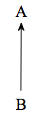
\includegraphics[height=.8in]{factoringI}}

\begin{itemize}
\tightlist
\item
  Bayesian networks specify how joint distributions are factored into
  conditional distributions using nodes to represent RV's and arrows to
  represent dependencies.
\item
  Nodes at the heads of arrows \emph{must} be on the left hand side of
  the conditioning symbols;
\item
  Nodes at the tails of arrows are on the right hand side of the
  conditioning symbols.
\item
  Any node at the tail of an arrow without and arrow leading into it
  must be expressed unconditionally.
\end{itemize}

\end{frame}

\begin{frame}{Factoring with DAGs}

\centerline{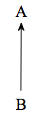
\includegraphics[height=.8in]{factoringI}}

\(\Pr(A,B) =\)

\end{frame}

\begin{frame}{Factoring with DAGs}

\centerline{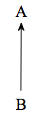
\includegraphics[height=.8in]{factoringI}}

\(\Pr(A,B) = \Pr(A|B) \Pr(B)\)

\end{frame}

\begin{frame}{Factoring with DAGs}

\centerline{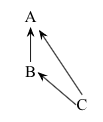
\includegraphics[height=.8in]{abcDag}}

\(\Pr(A,B,C) =\)

\end{frame}

\begin{frame}{Factoring with DAGs}

\centerline{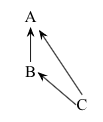
\includegraphics[height=.8in]{abcDag}}

\(\Pr(A,B,C) = \Pr(A|B,C)\Pr(B|C)\Pr(C)\)

\end{frame}

\begin{frame}{Work on lab}

Complete parts I-VI

\end{frame}

\end{document}
